\ifspanish

\question Las vv.aa. $S$ y $X$ obedecen a la ddp conjunta 
$$ p_{S,X}(s,x) = c, \quad 0<s<1, \; \;	  s<x<2s  $$
siendo $c$ una constante.
\begin{parts}
 		\part Tras representar el soporte de la ddp, calc\'{u}lese el valor de $c$.
		\part Establ\'{e}zcanse las expresiones de las ddp marginales $p_S(s)$ y $p_X(x)$.
		\part Determ\'{\i}nese anal\'{\i}ticamente la forma del estimador de error cuadr\'{a}tico medio m\'{\i}nimo de $S$ a la vista de $X$, $\hat{S}_\text{MSE}(X)$. Tr\'{a}cese dicha forma sobre la representaci\'{o}n del soporte de $p_{S,X}(s,x)$, y disc\'{u}tase si es posible determinarla directamente.
		\part Calc\'{u}lese el error cuadr\'{a}tico medio $\mathbb E\left\lbrace \left(S-\hat S_\text{MSE}(X)\right)^2 \right\rbrace $ que proporciona la aplicaci\'{o}n del estimador anterior.
		\part Determ\'{\i}nese la forma del estimador lineal de error cuadr\'{a}tico medio de $S$ a la vista de $X$, $\hat{S}_\text{LMSE}(X)$. Tr\'{a}cese dicha forma sobre la representaci\'{o}n del soporte de $p_{S,X}(s,x)$, y com\'{e}ntese su aspecto.
		\part Calc\'{u}lese el error cuadr\'{a}tico medio $\mathbb E\left\lbrace \left(S-\hat S_\text{LMSE}(X)\right)^2 \right\rbrace $  que proporciona la aplicaci\'{o}n del estimador anterior, y comp\'{a}rese con $\mathbb E\left\lbrace \left(S-\hat S_\text{MSE}(X)\right)^2 \right\rbrace $.
		\part ¿Qu\'{e} ocurre si se percibe (p.ej., visualizando muestras) que hay un comportamiento (estad\'{\i}stico) distinto para $0<X<1$ y $1<X<2$, y se dise\~{n}a un estimador lineal \'{o}ptimo diferente para cada uno de estos intervalos ($\hat{S}_{A,\text{LMSE}}(X)$ y $\hat{S}_{B,\text{LMSE}}(X)$, respectivamente)? Verif\'{\i}quese anal\'{\i}ticamente la soluci\'{o}n que se proponga.
\end{parts}

\begin{solution}
\begin{parts}
\part $c=2$; que puede obtenerse considerando que el \'{a}rea del soporte es 1/2.
\part $p_S(s)=2s, \; 0<s<1; \quad \quad p_X(x) =\left\{\begin{array}{ll}\displaystyle  
						  	  x &, 0<x<1\\
	  							2-x &, 1<x<2 
	 					 \end{array} 
						  \right. 
				      $
\part  $\;$ \\

 $ \hat{S}_\text{MSE}(X) =\left\{\begin{array}{ll}\displaystyle  
						  	  \frac{3X}{4}, & 0<X<1\\ \\ \displaystyle  
	  							\frac{1}{2}\left(\frac{X}{2}+1\right), & 1<X<2 
	 					 \end{array} 
						  \right. $
						  
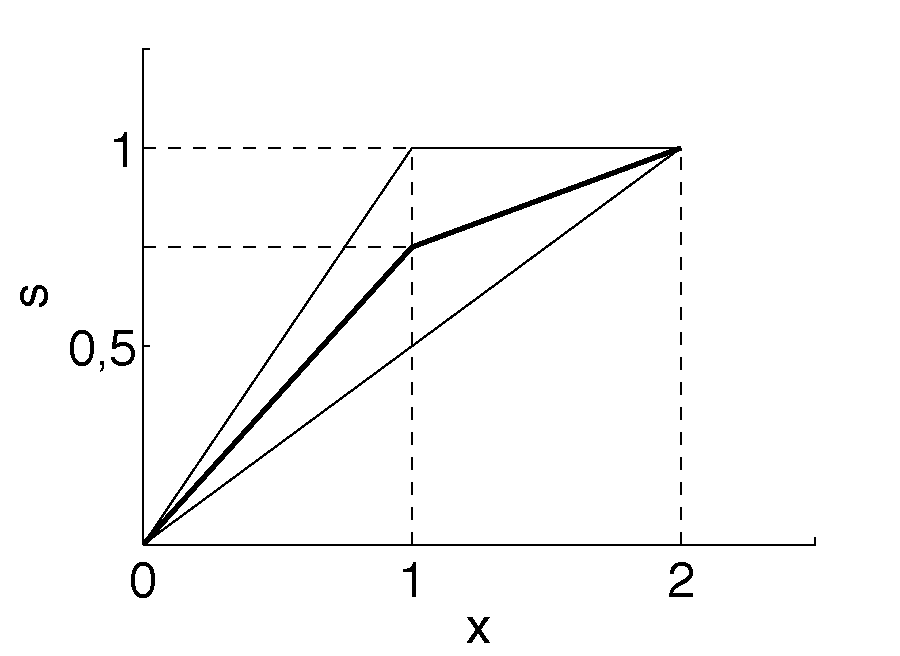
\includegraphics[width=6cm]{Figuras/fig22_1}
			     
%Podr\'{\i}a encontrarse directamente considerando que los cortes para $x$ se hacen sobre una distribuci\'{o}n uniforme, resultan los segmentos  promedio de los bordes.

Como los cortes para cada valor de $X$ se hacen sobre una ddp uniforme, resultan los segmentos promedio de los bordes.
\part $\mathbb E\left\lbrace \left(S-\hat S_\text{MSE}(X)\right)^2 \right\rbrace =\displaystyle\frac{1}{96}$
\part $\hat{S}_\text{LMSE}(X)=\displaystyle\frac{X}{2}+\displaystyle\frac{1}{6}$

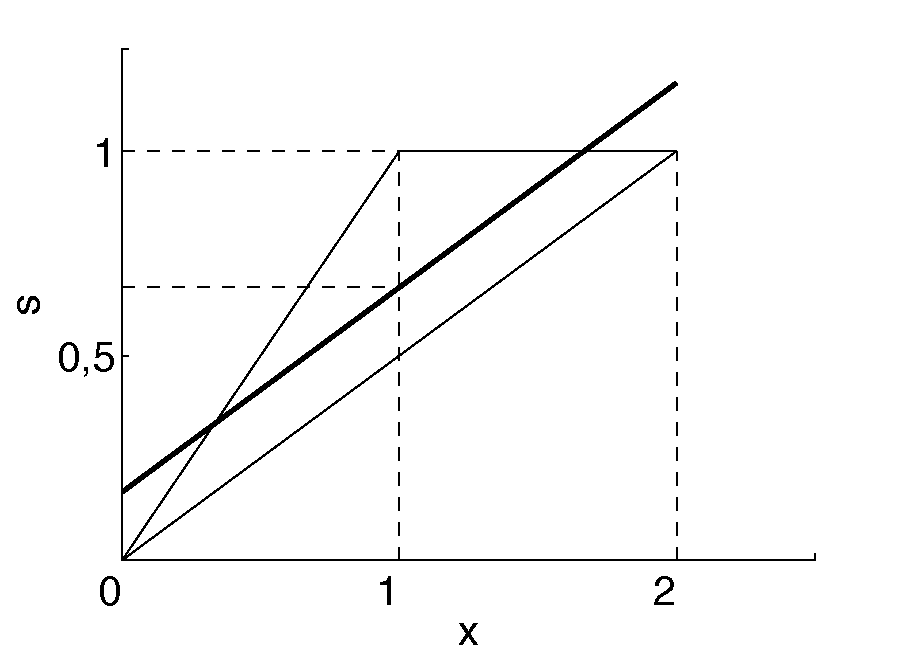
\includegraphics[width=6cm]{Figuras/fig22_2}
\part $\mathbb E\left\lbrace \left(S-\hat S_\text{LMSE}(X)\right)^2 \right\rbrace =\displaystyle\frac{11}{24}$; sensiblemente mayor que $\mathbb E\left\lbrace \left(S-\hat S_\text{MSE}(X)\right)^2 \right\rbrace $ 
\part $\hat{S}_{A,\text{LMSE}}(X)=\displaystyle\frac{3X}{4}$; $\hat{S}_{B,\text{LMSE}}(X)=\displaystyle\frac{1}{2}\left(\displaystyle\frac{X}{2}+1\right)$ que componen $\hat{S}_\text{MSE}(X)$.\\
%\includegraphics[width=6cm]{fig_1.eps}\\
$p_A(s,x)$ y $p_B(s,x)$ son uniformes, y los estimadores \'{o}ptimos lineales y de la forma anterior. 
 \end{parts}
\end{solution}

\else

\question Random variables $S$ and $X$ are characterized by the following joint distribution:
$$p_{S,X}(s,x) = c, \quad 0<s<1, \; \;	  s<x<2s  $$
with $c$ a constant.
\begin{parts}
 		\part Plot the support of the p.d.f., and use it to calculate the value of $c$.
		\part Give the expressions for the marginal p.d.f. of the random variables: $p_S(s)$ and $p_X(x)$.
		\part Find the minimum mean square error estimator of $S$ based on the observation of $X$, $\hat{S}_\text{MSE}(X)$. Plot the estimator on the same plot as the support of $p_{S,X}(s,x)$, and discuss whether it would had been possible to obtain the estimator without analytical derivations.
		\part Calculate the mean square error $\mathbb E\left\lbrace \left(S-\hat S_\text{MSE}(X)\right)^2 \right\rbrace $ incurred by the previous estimator.
		\part Now, find the linear minimum mean square error estimator of $S$ given $X$, $\hat{S}_\text{LMSE}(X)$. Again, plot the estimator together with the support of $p_{S,X}(s,x)$. Discuss your result.
		\part Obtain the mean square error $\mathbb E\left\lbrace \left(S-\hat S_\text{LMSE}(X)\right)^2 \right\rbrace $ of the linear estimator, and compare it with $\mathbb E\left\lbrace \left(S-\hat S_\text{MSE}(X)\right)^2 \right\rbrace $.
		\part It is perceived (e.g., visualizing several samples of $(X,S)$) that there exist different statistical behaviors for $0<X<1$ and $1<X<2$. What would occur if, based on this, different optimal linear estimators where designed for each of the intervals ($\hat{S}_{A,\text{LMSE}}(X)$ y $\hat{S}_{B,\text{LMSE}}(X)$, respectively)? Verify analytically the proposed solution.
\end{parts}

\begin{solution}
\begin{parts}
\part Since the area of the support of $p_{S,X}(s,x)$ is $1/2$, $c=2$.
\part $p_S(s)=2s, \; 0<s<1; \quad \quad p_X(x) =\left\{\begin{array}{ll}\displaystyle  
						  	  x &, 0<x<1\\
	  							2-x &, 1<x<2 
	 					 \end{array} 
						  \right. 
				      $
\part  $\;$ \\

 $ \hat{S}_\text{MSE}(X) =\left\{\begin{array}{ll}\displaystyle  
						  	  \frac{3X}{4}, & 0<X<1\\ \\ \displaystyle  
	  							\frac{1}{2}\left(\frac{X}{2}+1\right), & 1<X<2 
	 					 \end{array} 
						  \right. $
						  
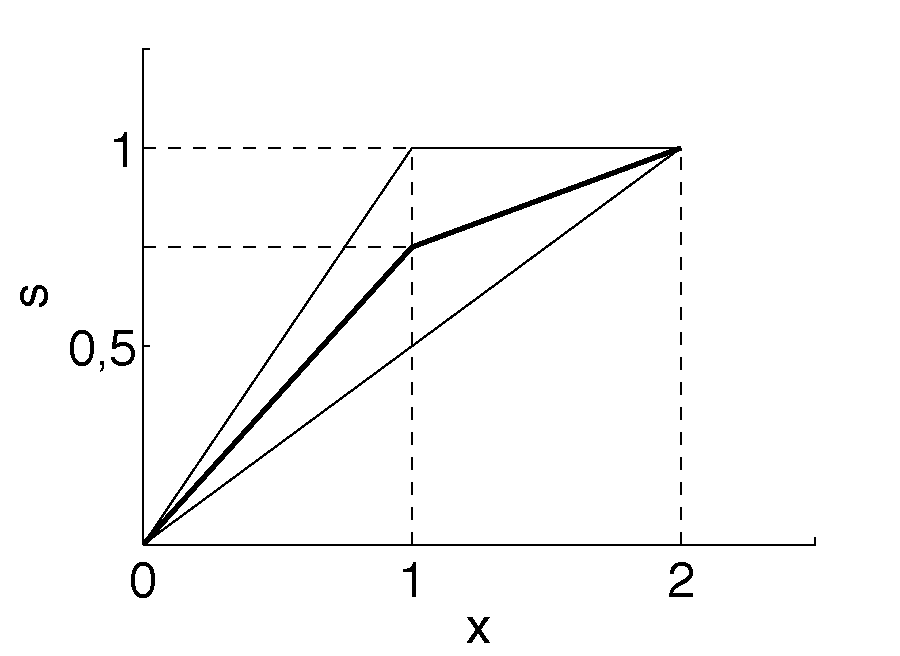
\includegraphics[width=6cm]{Figuras/fig22_1}
			     
%Podr\'{\i}a encontrarse directamente considerando que los cortes para $x$ se hacen sobre una distribuci\'{o}n uniforme, resultan los segmentos  promedio de los bordes.

Since for every value $X$ we have a uniform {\em a posteriori distribution} $p_{S|X}(s|x)$, the MSE estimator is given as the average between the minimum and maximum values of $S$ (for each $X$).
\part $\mathbb E\left\lbrace \left(S-\hat S_\text{MSE}(X)\right)^2 \right\rbrace =\displaystyle\frac{1}{96}$
\part $\hat{S}_\text{LMSE}(X)=\displaystyle\frac{X}{2}+\displaystyle\frac{1}{6}$

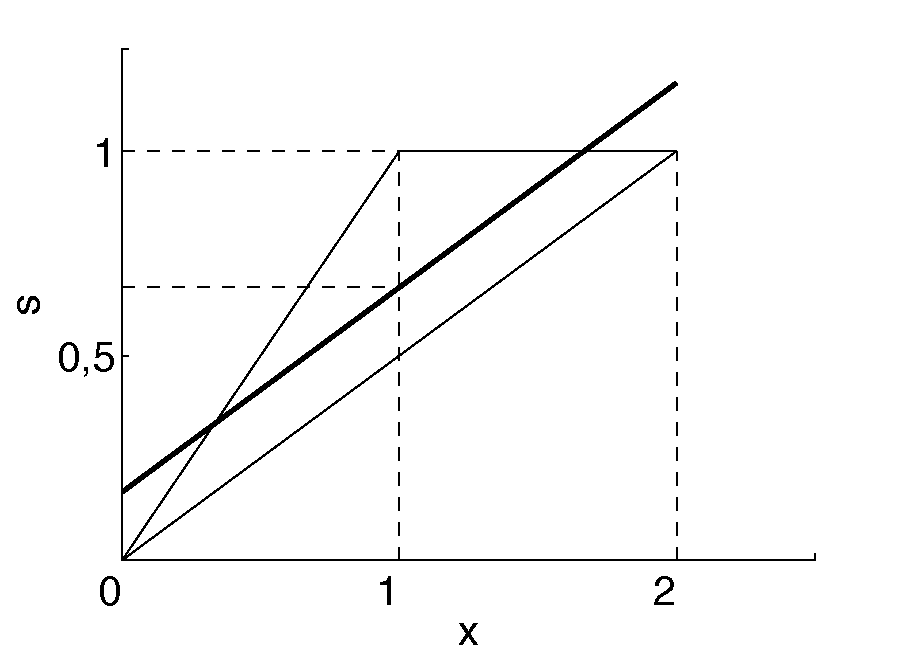
\includegraphics[width=6cm]{Figuras/fig22_2}
\part $\mathbb E\left\lbrace \left(S-\hat S_\text{LMSE}(X)\right)^2 \right\rbrace =\displaystyle\frac{11}{24}$, which is larger than $\mathbb E\left\lbrace \left(S-\hat S_\text{MSE}(X)\right)^2 \right\rbrace $ 
\part $\hat{S}_{A,\text{LMSE}}(X)=\displaystyle\frac{3X}{4}$ and $\hat{S}_{B,\text{LMSE}}(X)=\displaystyle\frac{1}{2}\left(\displaystyle\frac{X}{2}+1\right)$.  When jointly considered, these estimators compose $\hat{S}_\text{MSE}(X)$.\\
%\includegraphics[width=6cm]{fig_1.eps}\\
$p_A(s,x)$ and $p_B(s,x)$ are uniform, and now the linear estimators will also be optimal. 
 \end{parts}
 \end{solution}

\fi